\section{Implementation} \label{sec:implementation}

\nn{} was implemented based on an MSP430FR5994 development board.
Its runtime is implemented as a C library and used with function calls. 
\nn{} is available open-source at \textit{\url{https://git.soton.ac.uk/jz8u17/atom-energy}}, along with the simulation program of design exploration, comparisons of runtime (Samoyed and \debs{}), and benchmarks.
\todo[inline]{Check the git repo later.}

\begin{figure}[!t]
    \centering
    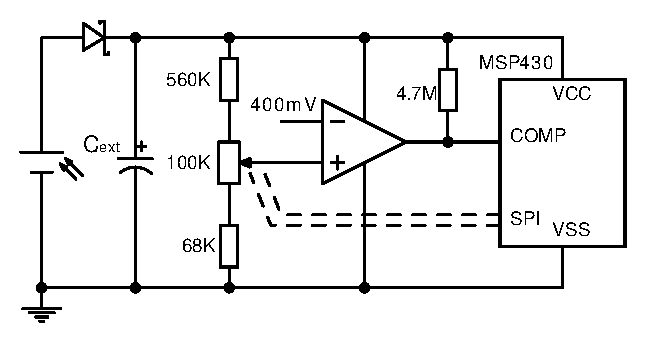
\includegraphics[width=0.8\columnwidth]{ch5_optic/figures/circuit_v2.pdf}
    \caption{\nn{} system schematic. }
    \label{fig:schematic}
\end{figure}

The system schematic is shown in \fref{fig:schematic}.
To reduce power consumption, the system utilises the MCU's on-chip ADC, timer, and voltage reference to perform energy profiling, and an external voltage monitor to monitor and control the threshold. 
The energy harvester is decoupled from the rest of the system by a diode to prevent the backflow of current when the harvester's power output drops off.
The harvested energy is then buffered in a \SI{10}{\micro\farad} capacitor (\nm{C}{ext}). 
Together with \SI{1.5}{\micro\farad} on-board decoupling capacitance, the system has an energy buffering capacity of \SI{11.5}{\micro\farad} in total. 


% Energy profiling hardware
The energy profiling is achieved through the on-chip modules.
The ADC reads voltage from a built-in 1/2 \nm{V}{cc} channel, and thus an external voltage divider is not needed. 
A \SI{2}{\volt} voltage reference is used by the ADC to convert the voltage reading, hence providing a \SIrange{0}{4}{\volt} reading range. 
A timer, driven by a \SI{10}{\kilo\hertz} low-power clock, records the charge and discharge cycle for \nn{}'s energy profiling.

\subsection{External Voltage Monitor}

As shown in \fref{fig:schematic}, we built an external voltage monitor to control the threshold that signals the MCU to wake up or sleep. 
The voltage monitor consists of a \SI{100}{\kilo\ohm} 129-step digital potentiometer (MCP4131-104) controlled through SPI, a voltage comparator (LT6703HVIS5-3) with \SI{400}{\milli\volt} internal reference. 
Two resistors, \SI{560}{\kilo\ohm} and \SI{68}{\kilo\ohm}, were connected with the digital potentiometer to provide a detection range of \SIrange{1.73}{4.28}{\volt}, which covers the operating voltage range of the system. 
A \SI{1}{\mega\ohm} pull-up resistor was added at the comparator's open-collector output.
Hence, the detected voltage threshold of \nm{V}{cc} is:
\begin{equation}
    \nmm{V}{th} = \frac{560 + 100 + 68}{\frac{\nmm{N}{wiper}}{128} * 100 + 68} \times 0.4 \quad(\SI{}{\volt})
    \label{eq:pot_thr}
\end{equation}
where \nm{N}{wiper} is the wiper step of the potentiometer, ranged in 0-128 inclusively. 
Also, the profiling result of $\Delta\nmm{V}{task}$ is stored as \nm{N}{profiling} in a digital ADC-scale format:
\begin{equation}
    \Delta\nmm{V}{task} = \frac{\nmm{N}{profiling}}{\nmm{N}{adcmax}} \times \nmm{V}{adcmax} 
    \label{eq:digit_profiling_result}
\end{equation}
where $\Delta\nmm{V}{task}$ is as defined in \eref{eq:vth_definition}. \nm{N}{adcmax} and \nm{V}{adcmax} are the maximum digital ADC reading and its corresponding voltage, which are 4095 and \SI{4}{\volt} respectively in our implementation.
Combining \eref{eq:vth_definition}, \eref{eq:pot_thr}, and \eref{eq:digit_profiling_result}, we can obtain the relationship between \nm{N}{profiling} and \nm{N}{wiper} as:
\begin{equation}
    \frac{\nmm{N}{profiling}}{\nmm{N}{adcmax}} \times \nmm{V}{adcmax} + \nmm{V}{end} = \frac{560 + 100 + 68}{\frac{\nmm{N}{wiper}}{128} * 100 + 68} \times 0.4
    \label{eq:adc_thr}
\end{equation}

where \nm{V}{end} is the target end voltage, which we set at \SI{2}{\volt} because the energy profiling  uses the \SI{2}{\volt} voltage reference for ADC reading such that the energy profiling can correctly work above \nm{V}{end}. 

In order to speed up the threshold setting from this non-linear relationship (\eref{eq:adc_thr}), We generated a look-up table to efficiently convert a profiling result \nm{N}{profiling} into the corresponding voltage threshold setting \nm{N}{wiper}. 
To avoid unnecessarily fine-grained steps, we equally divide \nm{N}{profiling} by a step of \nm{N}{step}. We recommend setting \nm{N}{step} as a power of 2 for an efficient threshold conversion, and we set \nm{N}{step} as 32, which translates to a voltage step of about \SI{31}{\milli\volt}.
We traversed \nm{N}{wiper} to find the closest \nm{V}{th} for each step of \nm{N}{profiling}, and the look-up table is then formed by the array of \nm{N}{wiper}. 
We also shifted the look-up table by one step higher so that the look-up table can inherently round up. 
Therefore, the corresponding threshold setting \nm{N}{wiper} of a profiling result \nm{N}{profiling} can be found in the look-up table with a computation-efficient index of $\frac{\nmm{N}{profiling}}{\nmm{N}{step}}$.

\subsection{Software}

\nn{}'s software is implemented as a library that accounts for the bootstrap configuration, function interfaces, memory mapping, and state retention. 
The bootstrap performs necessary system initialisation, such as configuring clocks, GPIOs, essential peripherals, and loading RAM data. 
\nn{}'s software interface is implemented as two function calls at the entry and exit of an atomic task. 
Each atomic task should be assigned with a function ID such that its state is independent from other atomic tasks. 
The state of an atomic task consists of a minimum of 2 bytes non-volatile data that accounts for a failure check and an adaptive threshold, with optional data for a user-defined control logic (e.g. a delay counter) or linear adaptation. 
The state retention mechanism is implemented as a style of reactive intermittent computing as in~\cite{balsamo2015hibernus, jayakumar2014quickrecall}.
The usage of \nn{}'s software is straightforward by assigning an ID to an atomic task in the library's header and calling the functions with the ID at the entry and exit of the atomic task. 
